% Student Number: 2240357068
% Student Name: Baturay KAFKAS
% EEE @ Hacettepe University

% Last update: 21:45 19/04/25

% My resource collection: https://github.com/kfksbtry/uni
% Circuits were set up in LTspice.

\documentclass{article}

\usepackage{comment}
\usepackage{graphicx}
\usepackage[top=25mm, bottom=25mm, left=25mm, right=25mm]{geometry}
\usepackage{amsmath}
\usepackage{moresize}
\usepackage{float}
\usepackage{fancyhdr}
\usepackage{booktabs}

\usepackage{pgfplots}
\pgfplotsset{width=10cm,compat=1.9}
\usepgfplotslibrary{external}
\tikzexternalize

\pagestyle{fancy}
\fancyhf{}
\fancyhead[R]{Baturay KAFKAS 2240357068 Electrical \& Electronics Engineering}

\rfoot{\thepage}
\renewcommand{\headrulewidth}{0pt}
\renewcommand{\footrulewidth}{0pt}

\setcounter{page}{30}

\begin{document}

\large

{\textit{This part of the experiment is prepared with Online LaTeX Editor Overleaf, and the circuits are drawn in LTspice. Visit the website for the code here:}}

{\textbf{https://www.overleaf.com/read/dcxnnrnyypxt\#b70098}}
\vspace{4mm}
\hrule
\vspace{4mm}
{\Large \textbf{1. PRELIMINARY WORK}}

\vspace{4mm}



{\textbf{1.1} Use source transformation to simplify the circuit given in Fig. 1 and obtain an 
equivalent circuit with respect to terminals a and b. Calculate the equivalent resistance 
between a and b (R$_{\text{ab}}$).}

\begin{figure}[H]
    \centering
    \includegraphics[width=0.5\linewidth]{msedge_l0mA0waTpo.png}
\end{figure}

\vspace{4mm}

{\textbf{Answer}: The two 220$\Omega$ resistors are in parallel, therefore the equivalent resistance is R$_\text{eq} = 220\Omega \ || \ 220\Omega = 110\Omega$. We may now transform the current source into a voltage source.}

\vspace{4mm}

{V$_\text{VS} = \text{I}_\text{CS} \cdot \text{R} = 10\text{mA} \cdot 110\Omega = 1.1\text{V} $}

\vspace{4mm}

\begin{figure}[H]
    \centering
    \includegraphics[width=0.75\linewidth]{Draft1.png}
\end{figure}

{The 110$\Omega$ and 100$\Omega$ resistors are in series, that is, R$_\text{eq} = 100\Omega \ + \ 110\Omega = 210\Omega$. Since two voltage sources, with their associated resistors, are in parallel, we may transform them into current sources.}

\vspace{4mm}

{I$\displaystyle _\text{left} = \frac{\text{V}_\text{left}}{\text{210}\Omega} = \frac{1.1\text{V}}{\text{210}\Omega} = 5.24\text{mA}$} \ \ \ {I$\displaystyle _\text{right} = \frac{\text{V}_\text{right}}{\text{120}\Omega} = \frac{11\text{V}}{\text{120}\Omega} = 91.7\text{mA}$}

\vspace{4mm}

\begin{figure}[H]
    \centering
    \includegraphics[width=0.8\linewidth]{Draft2.png}
\end{figure}

\vspace{4mm}

{The 210$\Omega$ and 120$\Omega$ resistors are in parallel. R$_\text{eq} = 210\Omega \ || \ 120\Omega = 76.36\Omega$. Two current sources can be merged.}

\vspace{4mm}

{I$_\text{CS} = (91.7 + 5.24)\text{mA} = 96.9\text{mA}$}

\vspace{4mm}

{Eventually, transform the current source into a voltage source.}

\vspace{4mm}

{V$_\text{VS} = 96.9\text{mA} \cdot 76.36\Omega = 7.4\text{V}$}

\vspace{4mm}

{The equivalent resistance becomes R$_\text{eq} = (76.36 + 330) \Omega = 406.36\Omega$}

\vspace{4mm}

\begin{figure}[H]
    \centering
    \includegraphics[width=0.75\linewidth]{Draft3.png}
\end{figure}

{$\boxed{\text{R}_\text{ab} = 406.36\Omega}$}

\vspace{8mm}

\newpage

{\textbf{1.2} For the circuit given in Fig. 2, calculate V$_{\text{ab}}$ and I$_{\text{ab}}$ for V$_{\text{in}}$ = 2V, 4V, 6V, 8V, and 10V. Sketch V$_{\text{ab}}$ vs. V$_{\text{in}}$ and comment on the plot.}

\begin{figure}[H]
    \centering
    \includegraphics[width=0.5\linewidth]{msedge_1dTlk624Fz.png}
\end{figure}

{\textbf{Answer}: Calculations and the graph are below.}

\vspace{4mm}

{V$\displaystyle _\text{in} = 2\text{V} \ \rightarrow \ \text{V}_\text{ab} = 2\text{V} \cdot \frac{330}{220 + 330} = 1.2\text{V} $} \ \ \ {$\displaystyle \text{I}_\text{ab} = \frac{2\text{V}}{(220 + 330)\Omega} = 3.63\text{mA} $}

\vspace{4mm}

{V$\displaystyle _\text{in} = 4\text{V} \ \rightarrow \ \text{V}_\text{ab} = 4\text{V} \cdot \frac{330}{220 + 330} = 2.4\text{V} $} \ \ \ {$\displaystyle \text{I}_\text{ab} = \frac{4\text{V}}{(220 + 330)\Omega} = 7.27\text{mA} $}

\vspace{4mm}

{V$\displaystyle _\text{in} = 6\text{V} \ \rightarrow \ \text{V}_\text{ab} = 6\text{V} \cdot \frac{330}{220 + 330} = 3.6\text{V} $} \ \ \ {$\displaystyle \text{I}_\text{ab} = \frac{6\text{V}}{(220 + 330)\Omega} = 10.9\text{mA} $}

\vspace{4mm}

{V$\displaystyle _\text{in} = 8\text{V} \ \rightarrow \ \text{V}_\text{ab} = 8\text{V} \cdot \frac{330}{220 + 330} = 4.8\text{V} $} \ \ \ {$\displaystyle \text{I}_\text{ab} = \frac{8\text{V}}{(220 + 330)\Omega} = 14.5\text{mA} $}

\vspace{4mm}

{V$\displaystyle _\text{in} = 10\text{V} \ \rightarrow \ \text{V}_\text{ab} = 10\text{V} \cdot \frac{330}{220 + 330} = 6.0\text{V} $} \ \ \ {$\displaystyle \text{I}_\text{ab} = \frac{10\text{V}}{(220 + 330)\Omega} = 18.1\text{mA} $}

\vspace{4mm}

\begin{center}
    \large
    \begin{tabular}{ |c| c c c c c | } 
    \hline
        V$_\text{in}$ (V) & 2 & 4 & 6 & 8 & 10\\
        \hline
        V$_\text{ab}$ (V) & 1.2 & 2.4 & 3.6 & 4.8 & 6.0 \\
        \hline
        I$_\text{ab}$ (mA) & 3.63 & 7.27 & 10.9 & 14.5 & 18.1 \\
        \hline
    \end{tabular}
\end{center}

\begin{center}
\begin{tikzpicture}

\begin{axis}[
    title={Graph 1: The relation between V$_\text{in}$ and V$_\text{ab}$},
    xlabel={V$_\text{in}$ (V)},
    ylabel={V$_\text{ab}$ (V)},
    xmin=2, xmax=10,
    ymin=1.2, ymax=6.0,
    xtick={2,4,6,8,10},
    ytick={1.2, 2.4, 3.6, 4.8, 6.0},
    legend pos=north west,
    ymajorgrids=true,
    xmajorgrids=true,
    grid style=dashed,
]

\addplot[
    color=blue,
    mark=square,
    ]
    coordinates {
    (2,1.2)(4,2.4)(6,3.6)(8,4.8)(10, 6.0)
    };

\end{axis}

\end{tikzpicture}
\end{center}

\vspace{4mm}

{The voltage across the resistor changes linearly in accordance with the voltage provided by the source.}

\vspace{8mm}

{\textbf{1.3} Current divider circuit in Fig. 3. Calculate I$_{\text{in}}$,  I$_1$, and I$_2$, for V$_{\text{in}}$ = 0.66V, 1.32V, 1.98V, 3.3V, and 3.64V. Sketch I$_{\text{in}}$ vs I$_1$ and I$_{\text{in}}$ vs I$_2$.}

\begin{figure}[H]
    \centering
    \includegraphics[width=0.5\linewidth]{msedge_5aVv5c0yu8.png}
\end{figure}

\vspace{4mm}

{\textbf{Answer}: Calculations and the graph are below.}

\vspace{4mm}

{R$\displaystyle _\text{eq} = 220\Omega \ || \ 330\Omega = 132\Omega $}

\vspace{4mm}

{V$\displaystyle _\text{in} = 0.66\text{V} \rightarrow  \text{I}_\text{in} = \frac{0.66\text{V}}{132\Omega} = 5\text{mA} $} \ \ \ {$\displaystyle \text{I}_\text{1} =  5\text{mA} \cdot\frac{\text{330}}{220 + 330} = 3\text{mA} $} \ \ \ {$\displaystyle \text{I}_\text{2} = 2\text{mA} $}

\vspace{4mm}

{V$\displaystyle _\text{in} = 1.32\text{V} \rightarrow  \text{I}_\text{in} = \frac{1.32\text{V}}{132\Omega} = 10\text{mA} $} \ \ \ {$\displaystyle \text{I}_\text{1} =  10\text{mA} \cdot\frac{\text{330}}{220 + 330} = 6\text{mA} $} \ \ \ {$\displaystyle \text{I}_\text{2} = 4\text{mA} $}

\vspace{4mm}

{V$\displaystyle _\text{in} = 1.98\text{V} \rightarrow  \text{I}_\text{in} = \frac{1.98\text{V}}{132\Omega} = 15\text{mA} $} \ \ \ {$\displaystyle \text{I}_\text{1} =  15\text{mA} \cdot\frac{\text{330}}{220 + 330} = 9\text{mA} $} \ \ \ {$\displaystyle \text{I}_\text{2} = 6\text{mA} $}

\vspace{4mm}

{V$\displaystyle _\text{in} = 3.3\text{V} \rightarrow  \text{I}_\text{in} = \frac{3.3\text{V}}{132\Omega} = 25\text{mA} $} \ \ \ {$\displaystyle \text{I}_\text{1} = 25\text{mA} \cdot\frac{\text{330}}{220 + 330} = 15\text{mA} $} \ \ \ {$\displaystyle \text{I}_\text{2} = 10\text{mA} $}

\vspace{4mm}

{V$\displaystyle _\text{in} = 3.64\text{V} \rightarrow  \text{I}_\text{in} = \frac{3.64\text{V}}{132\Omega} = 27.6\text{mA} $} \ \ \ {$\displaystyle \text{I}_\text{1} =  27.6\text{mA} \cdot\frac{\text{330}}{220 + 330} = 16.5\text{mA} $} \ \ \ {$\displaystyle \text{I}_\text{2} = 11.1\text{mA} $}

\vspace{4mm}

\begin{center}
    \large
    \begin{tabular}{ |c| c c c c c | } 
    \hline
        V$_\text{in}$ (V) & 0.66 & 1.32 & 1.98 & 3.3 & 3.64\\
        \hline
        I$_\text{in}$ (mA) & 5 & 10 & 15 & 25 & 27.6 \\
        \hline
        I$_\text{1}$ (mA) & 3 & 6 & 9 & 15 & 16.5 \\
        \hline
        I$_\text{2}$ (mA) & 2 & 4 & 6 & 10 & 11.1 \\
        \hline
    \end{tabular}
\end{center}

\vspace{4mm}

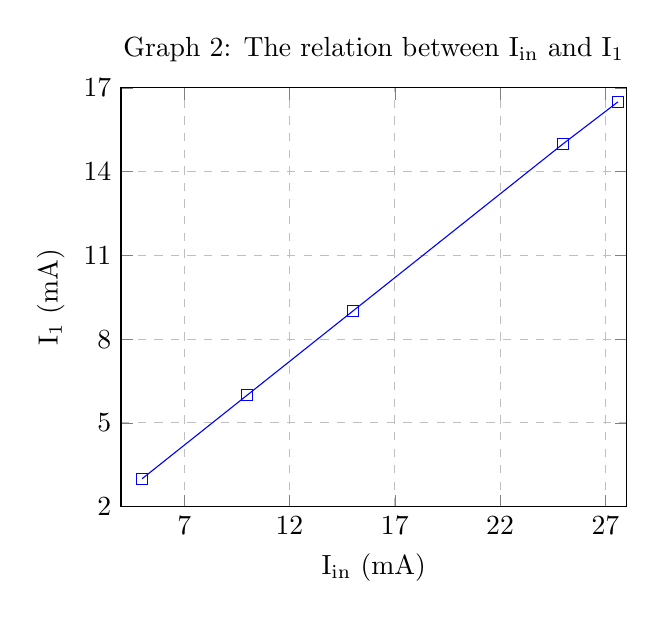
\begin{tikzpicture}

\begin{axis}[
    title={Graph 2: The relation between I$_\text{in}$ and I$_\text{1}$},
    width = 8cm,
    xlabel={I$_\text{in}$ (mA)},
    ylabel={I$_\text{1}$ (mA)},
    xmin=4, xmax=28,
    ymin=2, ymax=17,
    xtick={2, 7, 12, 17, 22, 27},
    ytick={2, 5, 8, 11, 14, 17},
    legend pos=north west,
    ymajorgrids=true,
    xmajorgrids=true,
    grid style=dashed,
]

\addplot[
    color=blue,
    mark=square,
    ]
    coordinates {
    (5,3)(10,6)(15,9)(25,15)(27.6, 16.5)
    };

\end{axis}

\vspace{4mm}

\end{tikzpicture}
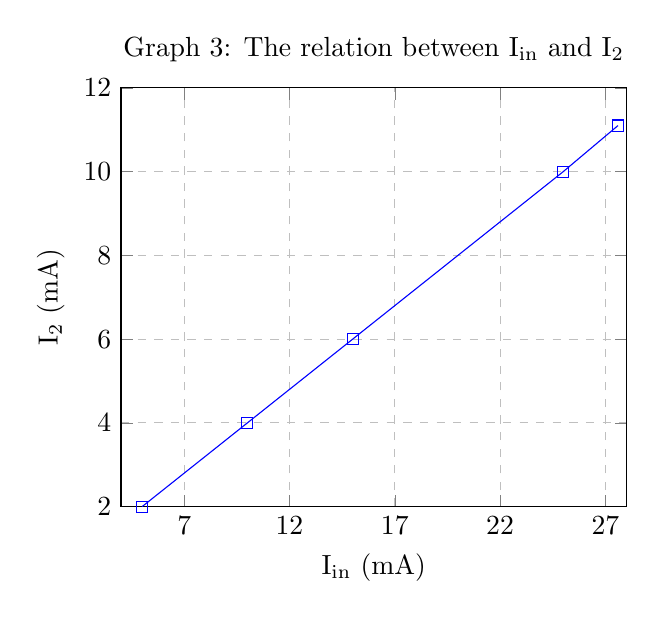
\begin{tikzpicture}

\begin{axis}[
    title={Graph 3: The relation between I$_\text{in}$ and I$_\text{2}$},
    width = 8cm,
    xlabel={I$_\text{in}$ (mA)},
    ylabel={I$_\text{2}$ (mA)},
    xmin=4, xmax=28,
    ymin=2, ymax=12,
    xtick={2, 7, 12, 17, 22, 27},
    ytick={2, 4, 6, 8, 10, 12},
    legend pos=north west,
    ymajorgrids=true,
    xmajorgrids=true,
    grid style=dashed,
]

\addplot[
    color=blue,
    mark=square,
    ]
    coordinates {
    (5,2)(10,4)(15,6)(25,10)(27.6, 11.1)
    };

\end{axis}

\end{tikzpicture}

\vspace{4mm}

{Similar to the answer in \textbf{1.2}, the relation between the currents is linear.}

\newpage

{\textbf{1.4} Using the superposition principle, find V$_{\text{ab}}$ given in Fig. 4.}

\begin{figure}[H]
    \centering
    \includegraphics[width=0.5\linewidth]{msedge_B4c8SxA7lv.png}
\end{figure}

\vspace{4mm}

{\textbf{Answer}: First, let's open-circuit the current source, then benefit from the voltage divider.}

\vspace{4mm}

\begin{figure}[H]
    \centering
    \includegraphics[width=0.75\linewidth]{Draft4.png}
\end{figure}

\vspace{4mm}

{V'$\displaystyle _\text{ab} = 10\text{V} \cdot \frac{100}{100+220+330} = 1.54\text{V}$}

\vspace{8mm}

{Second, we'll short-circuit the voltage source.}

\begin{figure}[H]
    \centering
    \includegraphics[width=0.75\linewidth]{Draft5.png}
\end{figure}

{The source transformation method, and the voltage divider afterwards, will help us solve the problem.}

\vspace{4mm}

{V$_\text{VS} = 10\text{mA} \cdot 220\Omega = 2.2\text{V}$}

\vspace{4mm}

\begin{figure}[H]
    \centering
    \includegraphics[width=0.75\linewidth]{Draft6.png}
\end{figure}

\vspace{4mm}

{V''$\displaystyle _\text{ab} = -2.2\text{V} \cdot \frac{100}{100+220+330} = -0.34\text{V}$}

\vspace{4mm}

{This time, we need to put a minus because the current enters from the other terminal of the resistor (passive sign convention).}

\vspace{4mm}

{Using the superposition theorem, we add up the individual responses of independent sources.}

\vspace{4mm}

{V$\displaystyle _\text{ab} = \text{V'}_\text{ab} + \text{V''}_\text{ab} = 1.54\text{V} - 0.34\text{V} = 1.2\text{V}$}

\vspace{4mm}

{$\displaystyle \boxed{ \text{V}_\text{ab} = 1.2\text{V}}$}

\end{document}